\documentclass[11pt]{article}

\usepackage[margin=1in]{geometry}
\usepackage{graphicx}
\usepackage{xfrac}

\setlength{\parindent}{0pt}

\begin{document}
\begin{minipage}[t]{0.3\textwidth}
  \strut\vspace*{-\baselineskip}\newline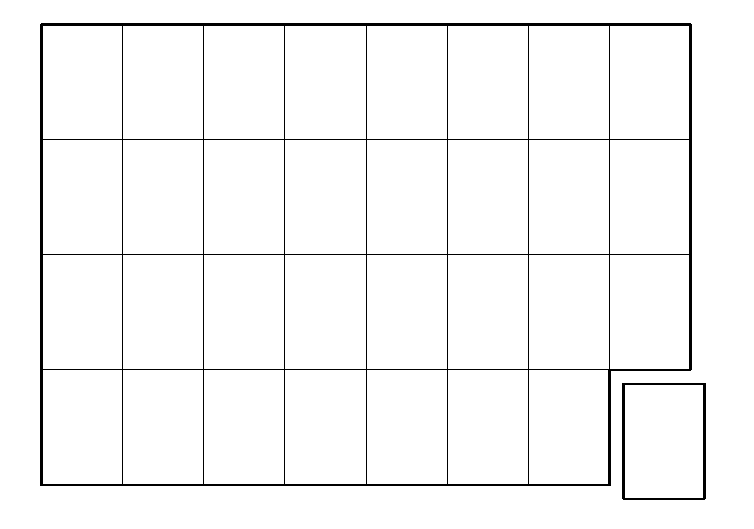
\includegraphics[width=\textwidth]{../figs/fig0}
  The starting proportions of paper control the relative ``thickness'' of the edges of the polyhedra.  I used a sheet of letter paper torn into 32 pieces.
\end{minipage}
\hspace{0.02\linewidth}
\begin{minipage}[t]{0.6\textwidth}
  {\Huge Wireframe Polyhedra Unit}
  \vspace*{0.25in}
  
  A set of folds to make units for all the Platonic, Archimedean, and Johnson solids with equal edge length.  The angles created are not necessarily exact, but are relatively straightforward to fold and practical if you want to fold the 1000+ units for the uniform solids.  Based on the fold for the ``Outline Dodecahedron'' in David Mitchell's {\bf Mathematical Origami}.
\end{minipage}

\vspace*{0.125in}

\begin{minipage}[t]{0.45\textwidth}
  \includegraphics[width=\textwidth]{../figs/fig1}
  \begin{itemize}{\item[1.] Crease the sheet into quarters.}\end{itemize}
\end{minipage}
\hfill
\begin{minipage}[t]{0.45\textwidth}
  \includegraphics[width=\textwidth]{../figs/fig2}
  \begin{itemize}{\item[2.] Make a small crease at the center of the sheet on the line made by bringing the lower left corner to the centerline and meeting the \sfrac{3}{4} vertical crease. Repeat with the upper right corner.}\end{itemize}
\end{minipage}

\vspace*{0.125in}

\begin{minipage}[t]{0.45\textwidth}
  \includegraphics[width=\textwidth]{../figs/fig3}
  \begin{itemize}{\item[3.] The distance between the two small creases is the unit length of the polyhedron edges.  From here, choose the two face shapes the edge shares.}\end{itemize}
\end{minipage}

\newpage
{\Large Triangle Edge} (Non-Platonic) (Internal angle of 60$^\circ$ ideal, 60$^\circ$ folded)
\vspace*{0.25in}

\begin{minipage}[t]{0.45\textwidth}
  \includegraphics[width=\textwidth]{../figs/fig03b-04}
  \begin{itemize}{\item[4.] Crease horizontally through the intersection of creases from step 2.}\end{itemize}
\end{minipage}
\hfill
\begin{minipage}[t]{0.45\textwidth}
  \includegraphics[width=\textwidth]{../figs/fig03b-05}
  \begin{itemize}{\item[5.] Tear across the crease.}\end{itemize}
\end{minipage}

\vspace*{0.5in}

\begin{minipage}[t]{0.45\textwidth}
  \includegraphics[width=0.85\textwidth]{../figs/fig03b-06}
  \begin{itemize}{\item[6.] Fold the lower left corner to the \sfrac{3}{4} vertical crease, going from the bottom centerline.}\end{itemize}
\end{minipage}
\hfill
\begin{minipage}[t]{0.45\textwidth}
  \includegraphics[width=0.85\textwidth]{../figs/fig03b-07}
  \begin{itemize}{\item[7.] Crease, taking notice that the corner created by the previous fold goes over the \sfrac{3}{4} vertical crease.}\end{itemize}
\end{minipage}

\vspace*{0.5in}

\begin{minipage}[t]{0.45\textwidth}
  \includegraphics[width=0.85\textwidth]{../figs/fig03b-08}
  \begin{itemize}{\item[8.] Unfold, rotate by 180$^\circ$ and fold the second side.}\end{itemize}
\end{minipage}
\hfill
\begin{minipage}[t]{0.45\textwidth}
  \includegraphics[width=0.85\textwidth]{../figs/fig03b-09}
  \begin{itemize}{\item[9.] Finished view of the bottom half when both sides are folded.  Crease the centerline.}\end{itemize}
\end{minipage}

\newpage
{\Large Triangle Edge} (Platonic) (Internal angle of 60$^\circ$ ideal, 60$^\circ$ folded)
\vspace*{0.25in}

\begin{minipage}[t]{0.3\textwidth}
  \includegraphics[width=\textwidth]{../figs/fig03-04}
  \begin{itemize}{\item[4.] Crease horizontally through the intersection of creases from step 2.}\end{itemize}
\end{minipage}
\begin{minipage}[t]{0.3\textwidth}
  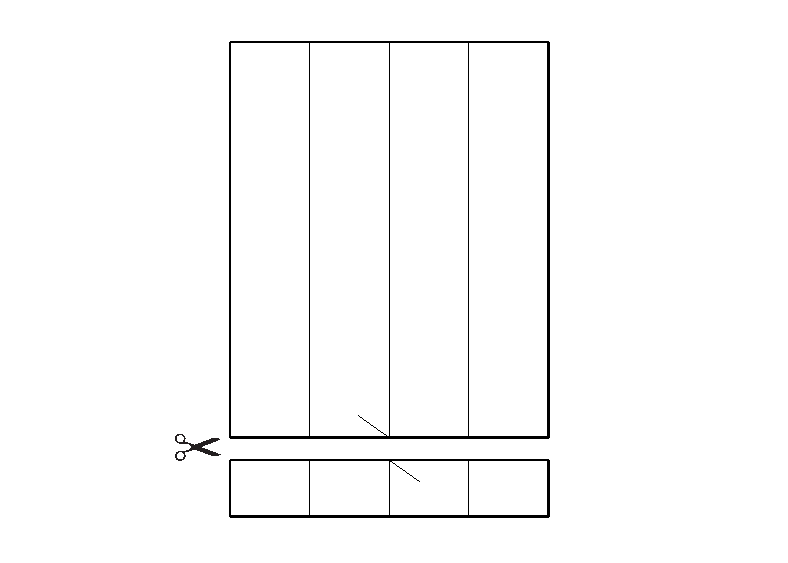
\includegraphics[width=\textwidth]{../figs/fig03-05}
  \begin{itemize}{\item[5.] Tear across the crease.}\end{itemize}
\end{minipage}
\begin{minipage}[t]{0.3\textwidth}
  \includegraphics[width=0.85\textwidth]{../figs/fig03-06}
  \begin{itemize}{\item[6.] Fold the lower left corner to the \sfrac{3}{4} vertical crease, going from the bottom centerline.}\end{itemize}
\end{minipage}

\vspace*{0.5in}

\begin{minipage}[t]{0.3\textwidth}
  \includegraphics[width=0.85\textwidth]{../figs/fig03-07}
  \begin{itemize}{\item[7.] Fold.}\end{itemize}
\end{minipage}
\begin{minipage}[t]{0.3\textwidth}
  \includegraphics[width=0.85\textwidth]{../figs/fig03-08}
  \begin{itemize}{\item[8.] Unfold, rotate by 180$^\circ$ and fold the second side.}\end{itemize}
\end{minipage}
\begin{minipage}[t]{0.3\textwidth}
  \includegraphics[width=0.85\textwidth]{../figs/fig03-09}
  \begin{itemize}{\item[9.] Finished view of the bottom half when both sides are folded.  Crease the centerline.}\end{itemize}
\end{minipage}

\newpage
{\Large Square Edge}  (Internal angle of 90$^\circ$ ideal, 90$^\circ$ folded)
\vspace*{0.25in}

\begin{minipage}[t]{0.3\textwidth}
  \includegraphics[width=\textwidth]{../figs/fig04-04}
  \begin{itemize}{\item[4.] Crease horizontally through the intersection of creases from step 2.}\end{itemize}
\end{minipage}
\begin{minipage}[t]{0.3\textwidth}
  \includegraphics[width=\textwidth]{../figs/fig04-05}
  \begin{itemize}{\item[5.] Fold the left edge where the crease from step 6 is to the centerline going though the intersection of creases from step 2.}\end{itemize}
\end{minipage}
\begin{minipage}[t]{0.3\textwidth}
  \includegraphics[width=\textwidth]{../figs/fig04-06}
  \begin{itemize}{\item[6.] Fold.}\end{itemize}
\end{minipage}

\vspace*{0.5in}

\begin{minipage}[t]{0.3\textwidth}
  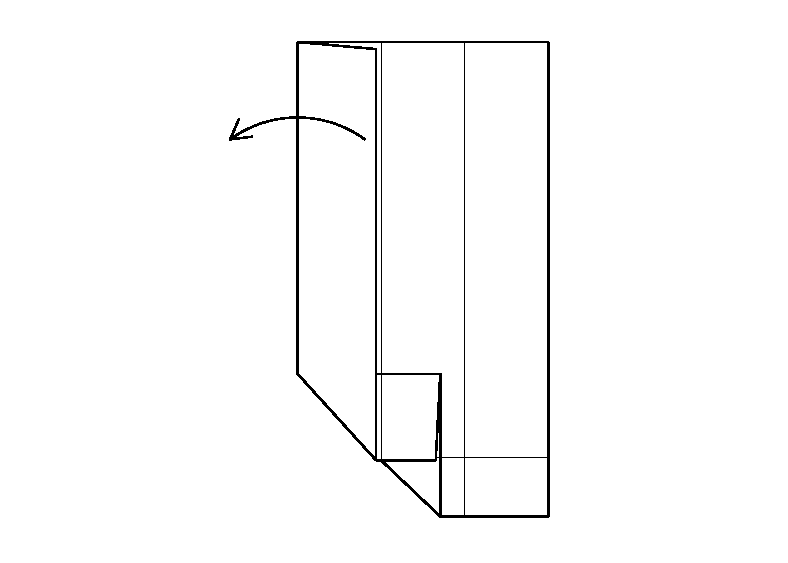
\includegraphics[width=\textwidth]{../figs/fig04-07}
  \begin{itemize}{\item[7.] Unfold, rotate by 180$^\circ$ and fold the second side.}\end{itemize}
\end{minipage}
\begin{minipage}[t]{0.3\textwidth}
  \includegraphics[width=\textwidth]{../figs/fig04-08}
  \begin{itemize}{\item[8.] Finished view of the bottom half when both sides are folded.  Crease the centerline.}\end{itemize}
\end{minipage}

\newpage
{\Large Pentagon Edge}  (Internal angle of 108$^\circ$ ideal, $\sim$109.5$^\circ$ folded)
\vspace*{0.25in}

\begin{minipage}[t]{0.3\textwidth}
  \includegraphics[width=\textwidth]{../figs/fig05-04}
  \begin{itemize}{\item[4.] Complete the full fold referenced in step 2.}\end{itemize}
\end{minipage}
\begin{minipage}[t]{0.3\textwidth}
  \includegraphics[width=\textwidth]{../figs/fig05-05}
  \begin{itemize}{\item[5.] Fold.}\end{itemize}
\end{minipage}
\begin{minipage}[t]{0.3\textwidth}
  \includegraphics[width=\textwidth]{../figs/fig05-06}
  \begin{itemize}{\item[6.] Unfold, rotate by 180$^\circ$ and fold the second side.}\end{itemize}
\end{minipage}

\vspace*{0.5in}

\begin{minipage}[t]{0.3\textwidth}
  \includegraphics[width=\textwidth]{../figs/fig05-07}
  \begin{itemize}{\item[7.] Finished view of the bottom half when both sides are folded.  Crease the centerline.}\end{itemize}
\end{minipage}

\newpage
{\Large Hexagon Edge} (Internal angle of 120$^\circ$ ideal, 120$^\circ$ folded)
\vspace*{0.25in}

\begin{minipage}[t]{0.3\textwidth}
  \includegraphics[width=\textwidth]{../figs/fig06-04}
  \begin{itemize}{\item[4.] Crease horizontally through the intersection of creases from step 2.}\end{itemize}
\end{minipage}
\begin{minipage}[t]{0.3\textwidth}
  \includegraphics[width=\textwidth]{../figs/fig06-05}
  \begin{itemize}{\item[5.] Fold the left edge where the crease from step 6 is to the \sfrac{1}{4} vertical crease going though the intersection of creases from step 2.}\end{itemize}
\end{minipage}
\begin{minipage}[t]{0.3\textwidth}
  \includegraphics[width=\textwidth]{../figs/fig06-06}
  \begin{itemize}{\item[6.] Fold.}\end{itemize}
\end{minipage}

\vspace*{0.5in}

\begin{minipage}[t]{0.3\textwidth}
  \includegraphics[width=\textwidth]{../figs/fig06-07}
  \begin{itemize}{\item[7.] Unfold, rotate by 180$^\circ$ and fold the second side.}\end{itemize}
\end{minipage}
\begin{minipage}[t]{0.3\textwidth}
  \includegraphics[width=\textwidth]{../figs/fig06-08}
  \begin{itemize}{\item[8.] Finished view of the bottom half when both sides are folded.  Crease the centerline.}\end{itemize}
\end{minipage}

\newpage
{\Large Octagon Edge} (Internal angle of 135$^\circ$ ideal, $\sim$137.6$^\circ$ folded)
\vspace*{0.25in}

\begin{minipage}[t]{0.3\textwidth}
  \includegraphics[width=\textwidth]{../figs/fig08-04}
  \begin{itemize}{\item[4.] Crease horizontally through the intersection of creases from step 2.}\end{itemize}
\end{minipage}
\begin{minipage}[t]{0.3\textwidth}
  \includegraphics[width=\textwidth]{../figs/fig08-05}
  \begin{itemize}{\item[5.] Fold the left corner to the \sfrac{1}{4} vertical crease going though the intersection of creases from step 2.}\end{itemize}
\end{minipage}
\begin{minipage}[t]{0.3\textwidth}
  \includegraphics[width=\textwidth]{../figs/fig08-06}
  \begin{itemize}{\item[6.] Fold.}\end{itemize}
\end{minipage}

\vspace*{0.5in}

\begin{minipage}[t]{0.3\textwidth}
  \includegraphics[width=\textwidth]{../figs/fig08-07}
  \begin{itemize}{\item[7.] Unfold, rotate by 180$^\circ$ and fold the second side.}\end{itemize}
\end{minipage}
\begin{minipage}[t]{0.3\textwidth}
  \includegraphics[width=\textwidth]{../figs/fig08-08}
  \begin{itemize}{\item[8.] Finished view of the bottom half when both sides are folded.  Crease the centerline.}\end{itemize}
\end{minipage}

\newpage
{\Large Dodecagon Edge} (Internal angle of 144$^\circ$ ideal, $\sim$141.1$^\circ$ folded)
\vspace*{0.25in}

\begin{minipage}[t]{0.3\textwidth}
  \includegraphics[width=\textwidth]{../figs/fig10-04}
  \begin{itemize}{\item[4.] Crease horizontally through the intersection of creases from step 2.}\end{itemize}
\end{minipage}
\begin{minipage}[t]{0.3\textwidth}
  \includegraphics[width=\textwidth]{../figs/fig10-05}
  \begin{itemize}{\item[5.] Fold going though the right corner and the intersection of creases from step 2.}\end{itemize}
\end{minipage}
\begin{minipage}[t]{0.3\textwidth}
  \includegraphics[width=\textwidth]{../figs/fig10-06}
  \begin{itemize}{\item[6.] Fold.}\end{itemize}
\end{minipage}

\vspace*{0.5in}

\begin{minipage}[t]{0.3\textwidth}
  \includegraphics[width=\textwidth]{../figs/fig10-07}
  \begin{itemize}{\item[7.] Unfold, rotate by 180$^\circ$ and fold the second side.}\end{itemize}
\end{minipage}
\begin{minipage}[t]{0.3\textwidth}
  \includegraphics[width=\textwidth]{../figs/fig10-08}
  \begin{itemize}{\item[8.] Finished view of the bottom half when both sides are folded.  Crease the centerline.}\end{itemize}
\end{minipage}

\end{document}
